\documentclass{standalone}
\usepackage{tikz,pgfplots}
\pgfplotsset{compat=1.18}
\begin{document}
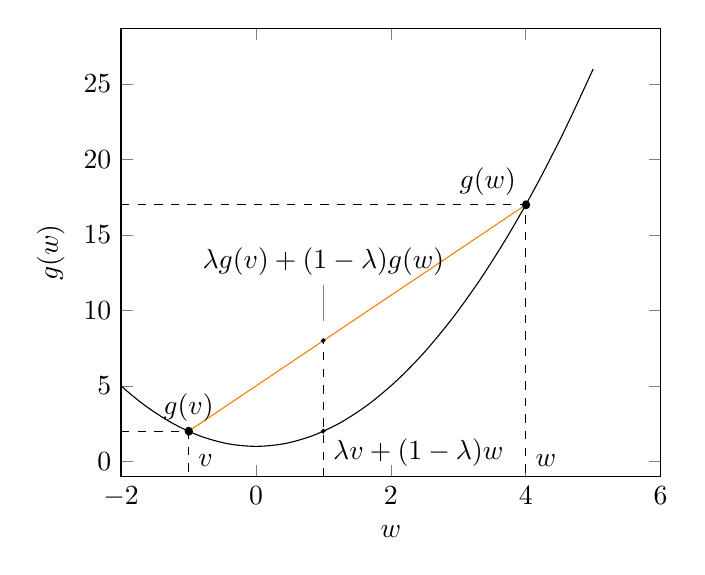
\begin{tikzpicture}
\begin{axis}[
        xlabel=$w$,
        ylabel=$g(w)$,
        xmin=-2,xmax=6,
        ymin=-1
        ]
    \addplot[smooth]{x^2+1};
    \draw[orange](-1,2)--(4,17);
    \draw[dashed](-2,2)--(-1,2)node[draw,circle,fill=black, inner sep=1pt]{}node[above]{$g(v)$}--(-1,-1)node[above right]{$v$};
    \draw[dashed](-2,17)--(4,17)node[draw,circle,fill=black, inner sep=1pt]{}node[above left]{$g(w)$}--(4,-1)node[above right]{$w$};
    \draw[dashed](1,-1)node[above right]{$\lambda v+(1-\lambda)w$}--(1,2)node[draw,circle,fill=black, inner sep=0.5pt]{}--(1,8)node[draw,circle,fill=black, inner sep=0.5pt]{}coordinate(a);
    \draw(a)node[above,pin=90:{$\lambda g(v)+(1-\lambda)g(w)$}]{};
\end{axis}    
\end{tikzpicture}
\end{document}